\pagestyle{fancy}

\graphicspath{ {Figures/Chapter5_SimulationBenchmarking/} }

The best way to crosscheck the reliability of the thermal evolution simulations introduced in the previous chapter is to compare them with experimental measurements. Many techniques have been developed for measuring the temperature evolution in objects \parencite[][]{ref:ThMeas1}. 

In our particular case, we were interested in measuring experimentally the temperature evolution of thin wires ($40 \mu m$) during their interaction with the beam of particles. However, no dedicated setup could be installed in any of the CERN machines. The only information available is the intensity registered by the detectors, so we needed to find a way to obtain the detector's temperature evolution from the registered intensity.  As explained in chapter \ref{ch:CurrentModeling} among the processes contributing to the current generation we have the Thermionic emission current ($J_{th}$). This contribution to the generated current is negligible at low temperatures but it becomes considerable when higher temperatures are reached. 

The idea for these measurements was to find certain beam conditions that allowed us to reach high temperatures and thus register the thermionic current. Due to the close relationship between the thermionic current and the temperature, by comparing the simulated current and the experimentally measured one, we could judge the reliability of our thermal simulation results. 

\section{Experimetnal Considerations}

Before starting with the experimental measurements we needed to first answer some questions: 

\subsection{Minimum detectable thermionic current}

For normal beam conditions, the currents measured by the individual wires in SEM grid, or the single wire in a Wire Scanner, are around 1 (mA). For the experimental planning, a signal was considered detectable if the thermionic current was higher than 0.05 (mA). Figure \ref{fig:ThermCurrent} shows the expected current generated in a Tungsten (40$\mu m$) and a Graphite (33 $\mu m$) wire as a function of the wire temperature. From this figure, one can observe that temperatures above 2100 (K) will be required to obtain a detectable thermionic current.  

\begin{figure}[h]
    \centering
    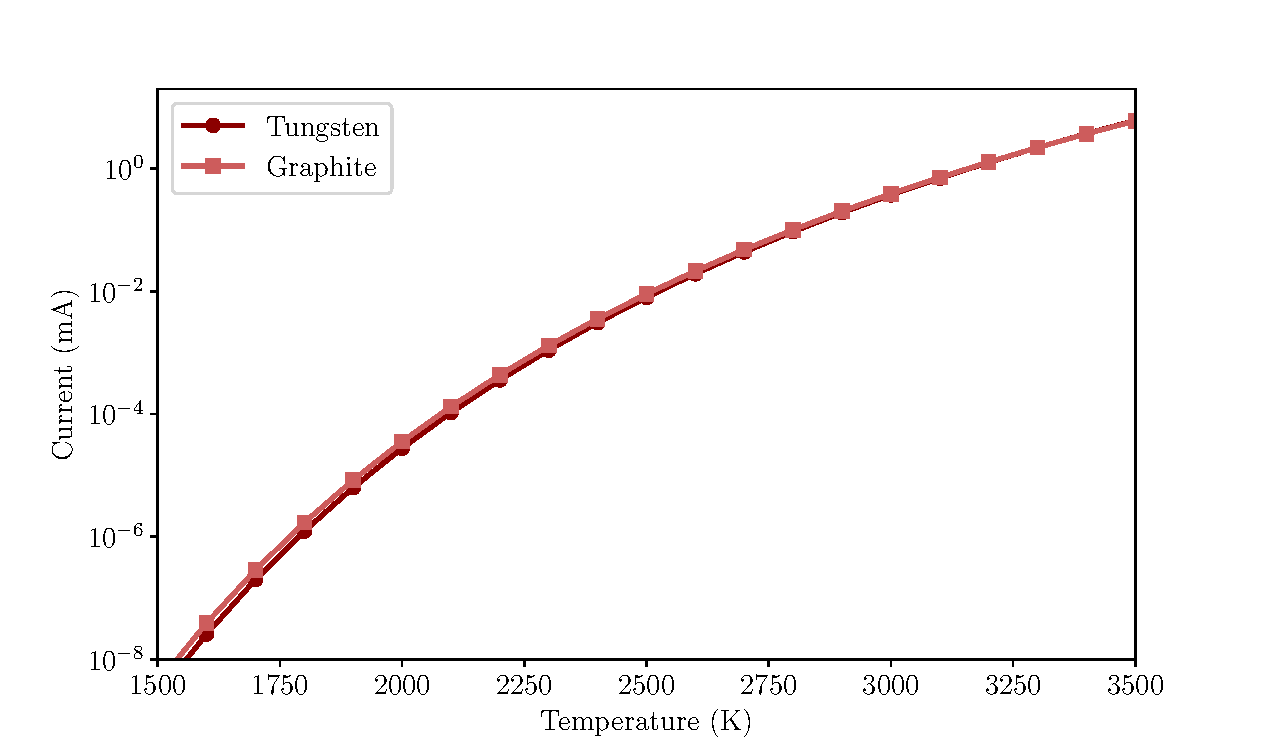
\includegraphics[width=0.80\columnwidth]{Figure_ThermoionicCurrent/ThermoCurrent.pdf}
    \caption{Thermionic current as a function of the temperature for Tungsten (40$\mu m$) and a Graphite (33 $\mu m$) wires.}
    \label{fig:ThermCurrent}
\end{figure}

\subsection{Available detectors}

Due to the high temperatures needed for performing the measurements, the risk of permanent detector damage was non-negligible. Only those detectors with already existing damage, or those placed in areas where the vacuum was intended to be disrupted could be used. 

After some deliberation, it was decided that the SEM grid L4T.BSGH/V.0243, would be used for the measurements. The beam current transformer L4T.BCT.0107 was used for continuous intensity and pulse length measurements. These detectors are located at LINAC4 in the L4T line, figure \ref{fig:DetLocation} shows the schematic representation of the location of the detector. 


\begin{figure}[h]
    \centering
    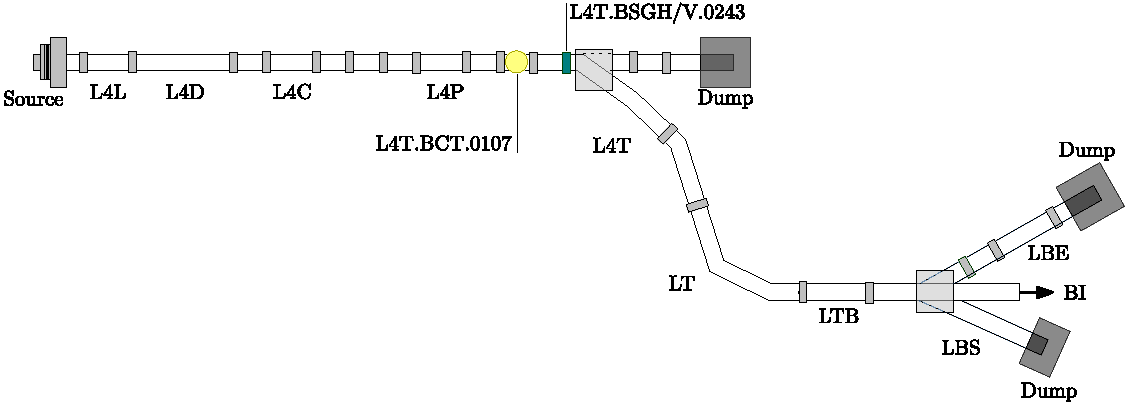
\includegraphics[width=0.90\columnwidth]{Figure_RelativePositionSemBCT/DetPosition.pdf}
    \caption{Schematic representation of Linac4 layout, with locations of the SEM Grid (L4T.BSGH/V.0243) and the BCT (L4T.BCT.0107) used for thermionic measurements.}
    \label{fig:DetLocation}
\end{figure}

The SEM grid used for the measurement was conformed of 32 Tungsten wires with gold coating. The wires had a length of 5 (cm) and a thickness of 40 $(\mu m)$. The wires were unevenly spaced, covering a total area of 40.9 (mm). Table \ref{tab:WireDist} details the locations of the different wires. The wires were placed on the top and the bottom part of the frame alternatively as shown in figure \ref{fig:WireLocation}.

\begin{table}[h]
    \centering
    \begin{tabular}{cccc}
    \hline
    Pitch              & \# of Wires & Wire Distance (mm) & Covered Region (mm) \\ \hline
    \multirow{5}{*}{3} & 6 + 6 = 12  & 0.4                & 4.4                 \\
                       & 3 + 3 = 6   & 0.75               & 8.9                 \\
                       & 3+3 = 6     & 1.0                & 14.9                \\
                       & 2 + 2 = 4   & 2.5                & 24.9                \\
                       & 2 + 2 = 4   & 4.0                & 40.9                \\ \hline
    \end{tabular}
    \label{tab:WireSpacing}
    \caption{Detailed description of wire location in SEM grid L4T.BSGH/V.0243}
\end{table}


\begin{figure}[h]
    \centering
    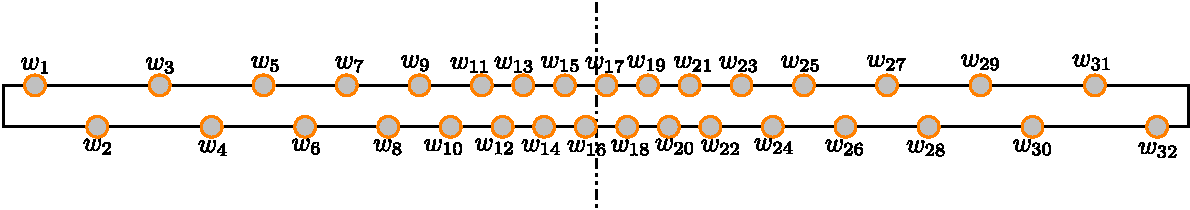
\includegraphics[width=0.90\columnwidth]{Figure_SemGridSchema/SemGridSchema.pdf}
    \caption{Schematic representation of wire position at L4T.BSGH/V.0243. }
    \label{fig:WireLocation}
\end{figure}

\subsection{Beam Conditions}

A preliminary study was performed to determine what kind of beam parameters would potentially yield a detectable thermionic current. In the L4T line, the energy of the \hm beam of particles is already 160 (MeV). The beam parameters that could be easily adjusted are: Beam intensity ($I_{beam}$), beam pulse length ($\Delta_t$), and beam size ($\sigma_x , \sigma_y$). Figure \ref{fig:Jth_Cond} shows a summary of the maximum expected thermionic current for different beam conditions. 

\begin{figure}[h]
    \centering
    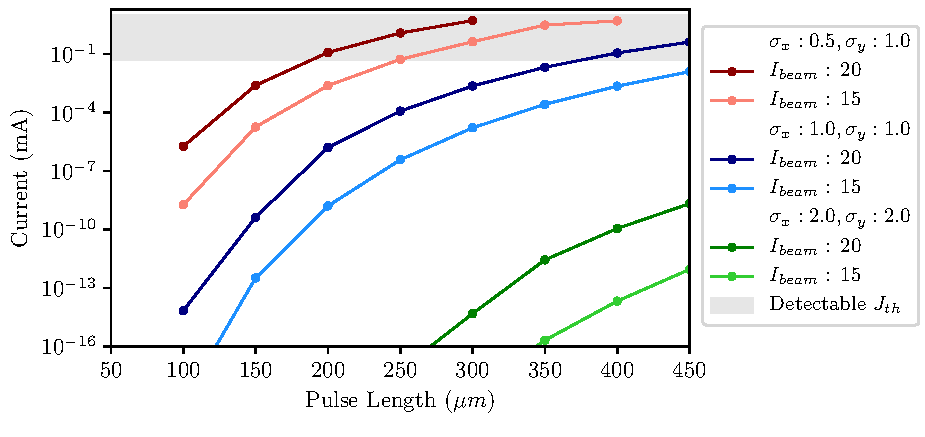
\includegraphics[width=0.90\columnwidth]{Figure_IsThereThermo/IsThereThermo.pdf}
    \caption{Summary of expected maximum current for different beam conditions. Gray Area indicates where thermionic emission is detectable. The beam size is given in (mm) and Beam intensity in (mA).}
    \label{fig:Jth_Cond}
\end{figure}

From this figure one can observe, that independently of the other beam conditions, large beam sizes ($\sigma_x = \sigma_y = 2 mm$) will not yield detectable thermionic emission. For smaller beam sizes ($\sigma_x \leq \sigma_y \leq 1 mm$), thermionic emission can be detected for long beam pulse lengths ($\Delta t > 300 \mu s$). Setting up the beam size to a specific dimension is not an easy task. Changes in the intensity of the beam also didn't produce very dramatic changes in the detectable current. During the measurements, these two quantities were kept constant while the beam pulse length was systematically increased in order to reach the thermionic stage in a controlled way. 

\section{Experimental Results}

The first set of measurements was taken using conservative beam conditions. The intensity of the beam was kept constant to $I_{beam} = 17.30 (17) mA$. Figure \ref{fig:PulseEvol} shows the evolution of the beam size during the first set of measurements. From this figure, we can see that the beam size was $\sigma_x = 1.02(5) mm$ and $\sigma_y = 1.76(2)$ mm. While the beam position remained constant around $\mu_x = -0.22(6) mm$ and $\mu_y = -0.43(21) mm$. 

\begin{figure}[h]
    \centering
    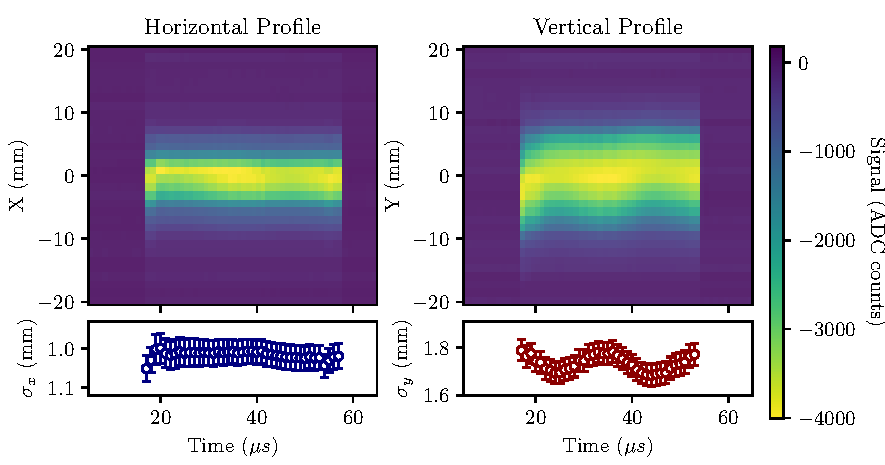
\includegraphics[width=1.0\columnwidth]{Figure_BeamProfileStudy/BeamProfEvol1.pdf}
    \caption{Evolution of the transverse beam profile along the beam pulse. Top: example of transverse beam profile measurement. Bottom: Calculated beam size from gaussian approximation. Error bars were calculated by measuring different beam pulses.  }
    \label{fig:PulseEvol}
\end{figure}

During these measurements, the beam pulse length was varied between $\Delta t = 165.38(48) \mu s$ up to $\Delta t = 247.12(33) \mu s$. As expected, no sign of thermionic emission was observed. However, when the long beam pulse lengths were measured, wires 15 and 17 were glued together. Figure \ref{fig:WireGlued} shows the current registered by the different wires as a function of time for six consecutive beam pulses. From this figure, we can see how after pulse 4, the currents registered by wires 15 and 17 are identical, indicating the wire attachment. 

\begin{figure}[h]
    \centering
    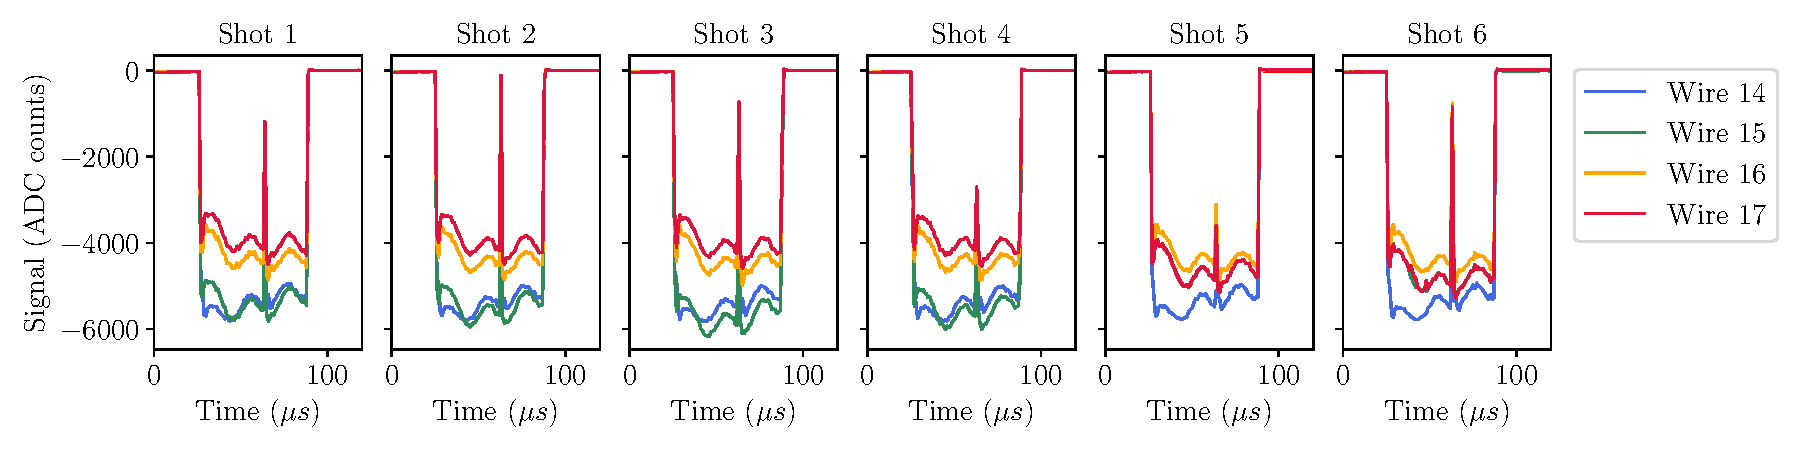
\includegraphics[width=1.0\columnwidth]{Figure_WiresGluing/WireWithTime.pdf}
    \caption{Evolution of the measured current in different wires as a function of time, for six consecutive beam pulses. }
    \label{fig:PulseEvol}
\end{figure}

In order to avoid this situation and proceed with the measurements, the beam of particles was steered away from these wires and centered around $\mu_x = -1.89(11) mm$ and $\mu_y = 1.15(31) mm$. The wire separation in this position is much larger, making wire gluing more challenging. 

To reach higher temperatures and to be able to reach the thermionic regime, the horizontal beam size was reduced to $\sigma_x = 0.59(17) mm$. As a result the vertical plane grew longer, $\sigma_y = 3.23(54) mm$. During these measurements, the beam intensity was sligtly smaller $I_{beam} \sim 16.7 mA$. The beam pulse length was increased systematically. On the vertical grid, Thermionic emission was observable in various wires for a beam pulse length of $\sim 450 \mu s$. 

\begin{figure}[h]
    \centering
    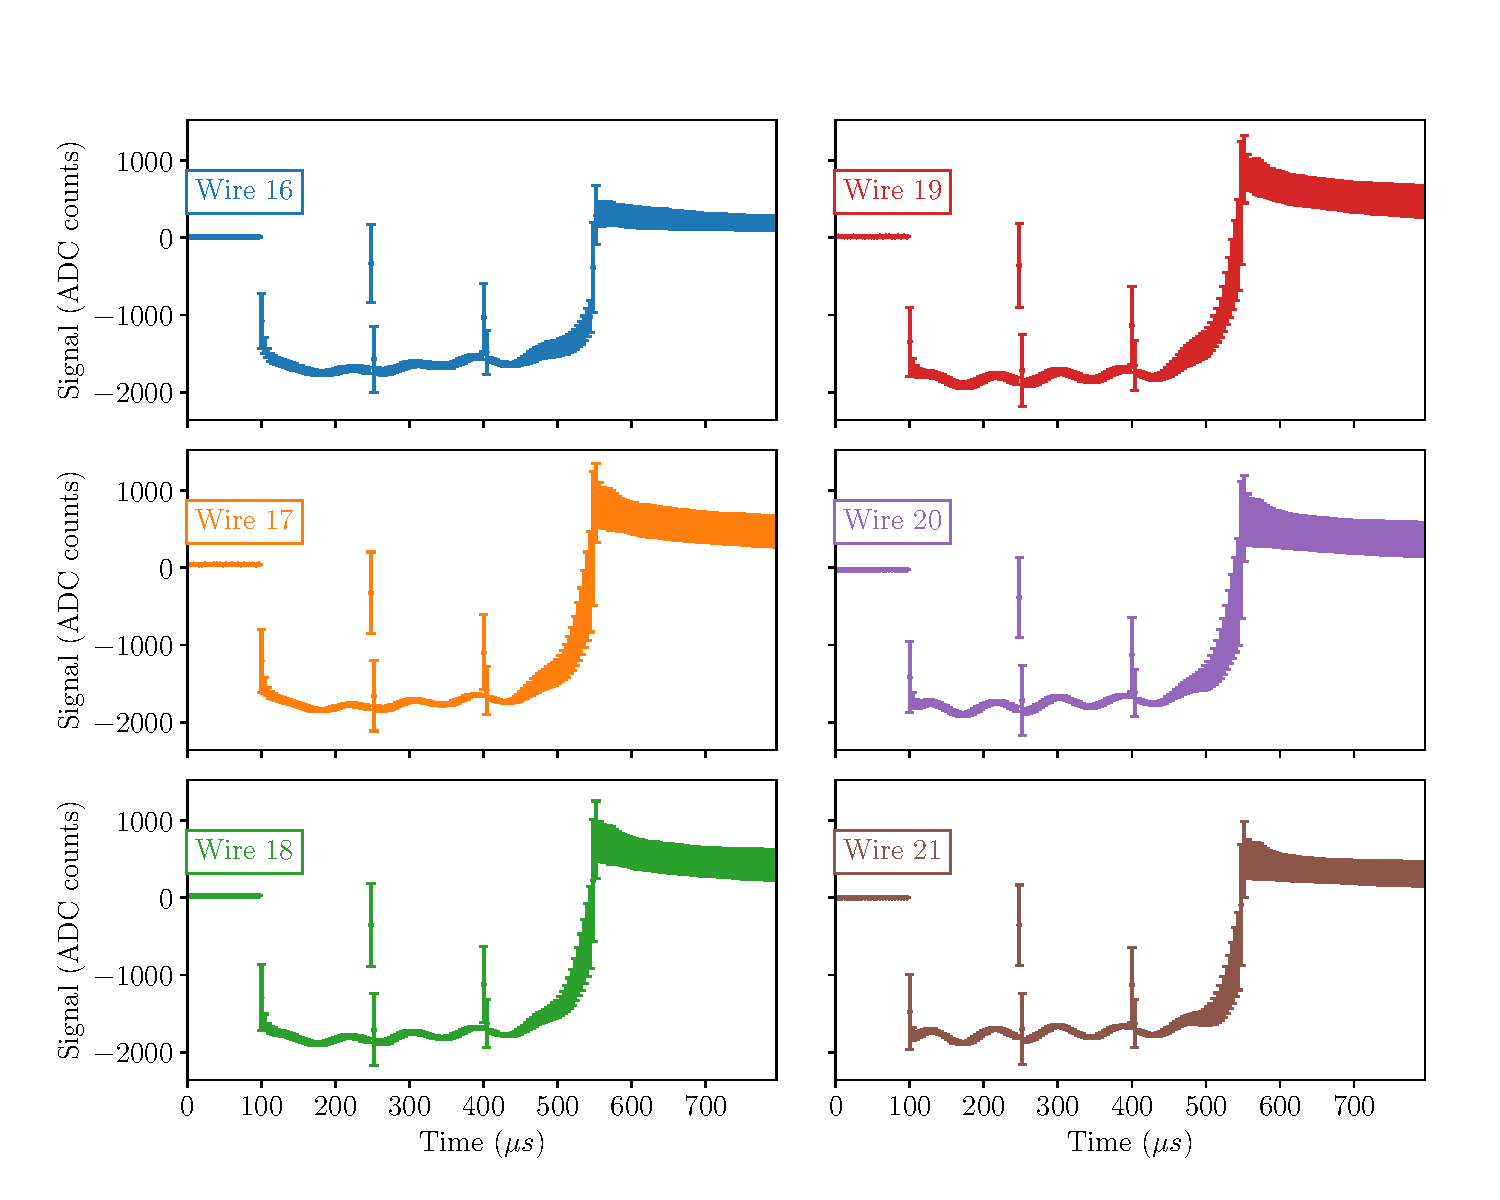
\includegraphics[width=0.9\columnwidth]{Figure_ThermionicMeasurements/VerticalThermoCurrent.pdf}
    \caption{Current registered by several wires during the beam pulse.}
    \label{fig:MeasuredThermo}
\end{figure}

Figure \ref{fig:MeasuredThermo} shows the current measured by several wires in the vertical SEM grid during the beam passage. From this figure, we can observe when the particle beam reaches the detector since a negative signal starts to be registered. As time goes by, the energy deposition in the detector material rises the temperature of the detector. As temperature increases, thermionic emission increases, and one can observe this increase in the reduction of the absolute value of the current. Once the particle beam has disappeared, a small positive current remains, because the detector is still warm, thermionic emission current is still being registered.  As the detector cools down, this current diminishes. 

In figure \ref{fig:MeasuredThermo} one can also observe some fluctuations in the registered beam current. This was an effect of the particle beam of particles itself, and could also be observed in the BCT measurements. Also, at $t = 250 \mu s$ and $t = 400 \mu s$, an anomalous value of the beam current is registered by all the wires. To avoid injection losses due to in-between rings injection, the Linac4 chopper removes part of the Linac4 beam every 150 $\mu s$. Which explains the intensity jumps registered by the wires. 

\begin{figure}[h]
    \centering
    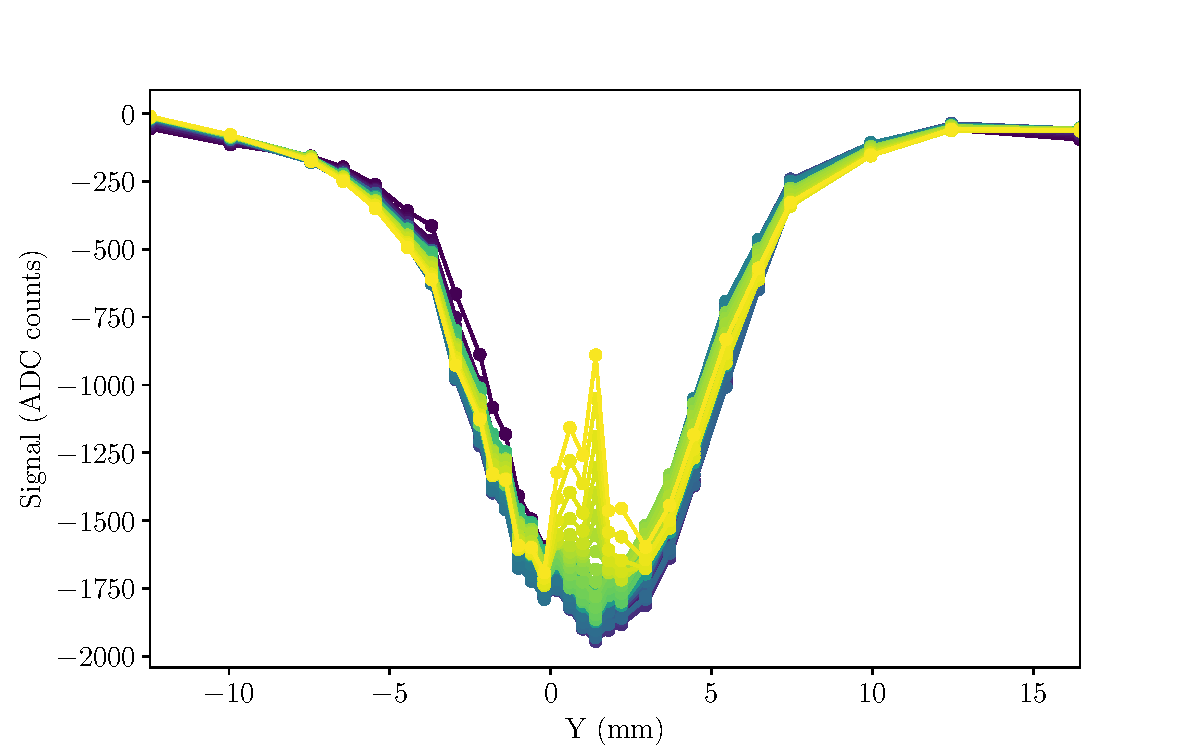
\includegraphics[width=0.75\columnwidth]{Figure_ThermionicMeasurements/ProfileJth.pdf}
    \caption{Example of vertical profile beam measurement. Darker colors indicate measurements at the beginning of the beam shot. Lighter colors indicate measurements a the end of the shot. }
    \label{fig:JthInProf}
\end{figure}

Figure \ref{fig:JthInProf} shows how thermionic emission affects the transverse beam profile measurements. In this figure, lighter currents indicate profiles taken at larger times during the beam pulse. Also from this image, we can see the absolute value of the current in the central wires diminishing as time goes by. 

\section{Measurment-Simulation Comparison}

PyTT program was used to simulate the thermal and electrical evolution of the detectors during the measurements. Figure \ref{fig:MeasSimCompa} shows a comparison between the current measured by wire 19 of the SEM grid, the simulated current, and the current measured by BCT.0107. The BCT intensity has been included in the comparison to show the intrinsic properties of the beam.

From this signal, the aforementioned beam intensity fluctuations and the chopper gaps can be also observed in the BCT measurement. However, the current reduction at longer beam pulse time is not observable in the BCT measurements, as this is an effect occurring on the wire. Also, the BCT measurement clearly shows when the beam pulse ends, proving that the positive current measured by the wire grid is not coming from the beam. 

\begin{figure}[h]
    \centering
    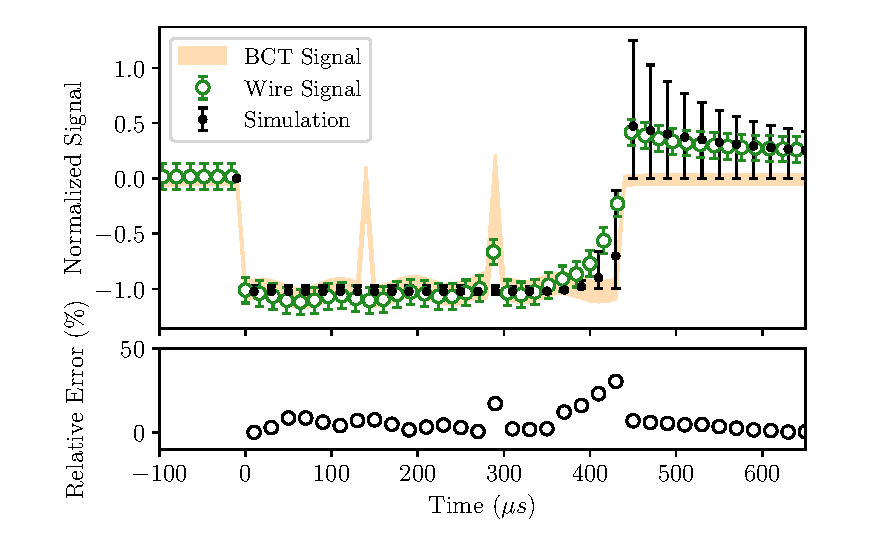
\includegraphics[width=0.75\columnwidth]{Figure_MeasurementSimulationCompa/VerticalCompa.pdf}
    \caption{Signal generated in the wire intercepting the beam as a function of time. Compared with simulated intensity results. }
    \label{fig:MeasSimCompa}
\end{figure}

Intra-pulse intensity fluctuations and chopper effects were not considered in the simulations. A constant current of $I_{beam} = 16.7 (mA)$ was considered. The simulation results seem to very clearly reproduce the average of the measured SEM current. The simulations show a slightly slower start for the thermionic emission current. However, after the beam pulse is gone, the simulated and the measured results for the thermionic current match very well. 

The maximum relative error between simulated and measured results is found to be around 30 $\%$, and it is found at the very end of the beam shot. Even then, the average relative error along the whole pulse is $6.3(25) \%$. 

A dedicated uncertainty study was performed to determine the uncertainties of the simulated results (See Section \ref{sec:ModelUnc}). In this particular case, the biggest contributor to the simulation's uncertainty came from uncertainties in the beam size. As indicated in the previous section, the beam size was $\sigma_x = 0.59(17) mm$ and $sigma_y = 3.23(54) mm$. This implies, beam size uncertainty was $\xi_x = 28.81 \%$ and $\xi_y = 16.71 \%$. As shown in section \ref{sec:ModelUnc}, uncertainties in beam sizes can yield big uncertainties in simulation results, mainly when small beam sizes are involved. 

As we saw in figure \ref{fig:MeasuredThermo}, several wires measured thermionic emission. However, due to the small changes in the measured intensity between the different wires and the big uncertainties in the simulated results, it was impossible to distinguish among them. 



